\paragraph{} 


\begin{table}
    \centering
    \newcommand\tableTop{\rule{0pt}{3ex}}
    \newcommand\tableMid{\rule{0pt}{3ex}}
    \newcommand\tableBottom{\rule[-2ex]{0pt}{0pt}}
    \newcolumntype{N}{>{\centering\arraybackslash}m{2.5in}}
    
    \renewcommand\theadfont{\normalsize}
    \renewcommand\arraystretch{1.3}
    \begin{tabular}{l@{\hskip 0.15in} r@{\hskip 0.6in} r@{\hskip 0.35in} r} 
        
        \toprule
        & \thead{\multirow{2}{*}{\textsc{Native}}} & \multicolumn{2}{c}{\thead{\textsc{Citadel}}} \\
        \cline{3-4}
        &  & \thead{\textit{Amortised}} & \thead{\textit{Cache Miss}} \\
        % \cline{1-4}
        \midrule 
        \texttt{open()} & $1.675\pm0.076$ & $6.083\pm0.129$ & $50.133\pm1.482$ \\
        \texttt{read()} & $5.724\pm0.206$ & $7.010\pm0.192$ & $54.736\pm1.556$ \\
        \texttt{write()} & $14.340\pm0.208$ & $15.597\pm0.250$ & $63.824\pm1.902$ \\
        \texttt{close()} & $0.651\pm0.005$ & \multicolumn{2}{c}{$0.718\pm0.011$} \\

        

        \midrule 
        \texttt{socket()} & $1.446\pm0.179$ & \multicolumn{2}{c}{$3.156\pm0.291$} \\
        \texttt{bind()} & $0.762\pm0.023$ & $1.911\pm0.183$ & $49.110\pm1.746$ \\
        \texttt{listen()} & $0.705\pm0.015$ & $1.882\pm0.149$ & $48.411\pm1.386$ \\
        \texttt{connect()} & $16.570\pm0.278$ & $17.961\pm0.330$ & $66.273\pm2.147$ \\

        \midrule 
        \texttt{shmget()} & $1.880\pm0.122$ & $1.913\pm0.111$ & $49.326\pm1.466$ \\
        \texttt{shmat()} & $0.420\pm0.005$ & $1.575\pm0.134$ & $47.997\pm1.560$ \\
        \texttt{shmctl()} & $0.418\pm0.005$ & $0.743\pm0.083$ & $45.912\pm1.114$ \\
        \texttt{shmdt()} & $0.415\pm0.003$ & \multicolumn{2}{c}{$1.342\pm0.040$} \\



        \midrule 
        \texttt{pipe()} & $1.110\pm0.061$ & $1.288\pm0.069$ & $47.334\pm1.147$ \\
        \texttt{mkfifo()} & $3.865\pm0.048$ & $11.509\pm0.405$ & $59.623\pm1.788$ \\

        \midrule 
        \texttt{fork()} & $47.866\pm3.175$ & $48.647\pm3.457$ & $81.174\pm3.829$ \\
        \texttt{citadel\_init()} & $-$ & $0.801\pm0.009$ & $34.940\pm1.329$ \\
        \bottomrule
    \end{tabular}
    \vspace{5mm}
    \captionsetup{justification=centering}
    \caption[\texttt{libcitadel} microbenchmarks]{\texttt{libcitadel} microbenchmarks. \\ All values are in $\mu s$ and the sample standard deviation is shown alongside the mean. For \textsc{Citadel}, both the amortised and average cache-miss durations are given. Only one value is given if the operation is not affects by a cache miss. $n=10^6$.}
\end{table}

\begin{figure}[]
    \centering
    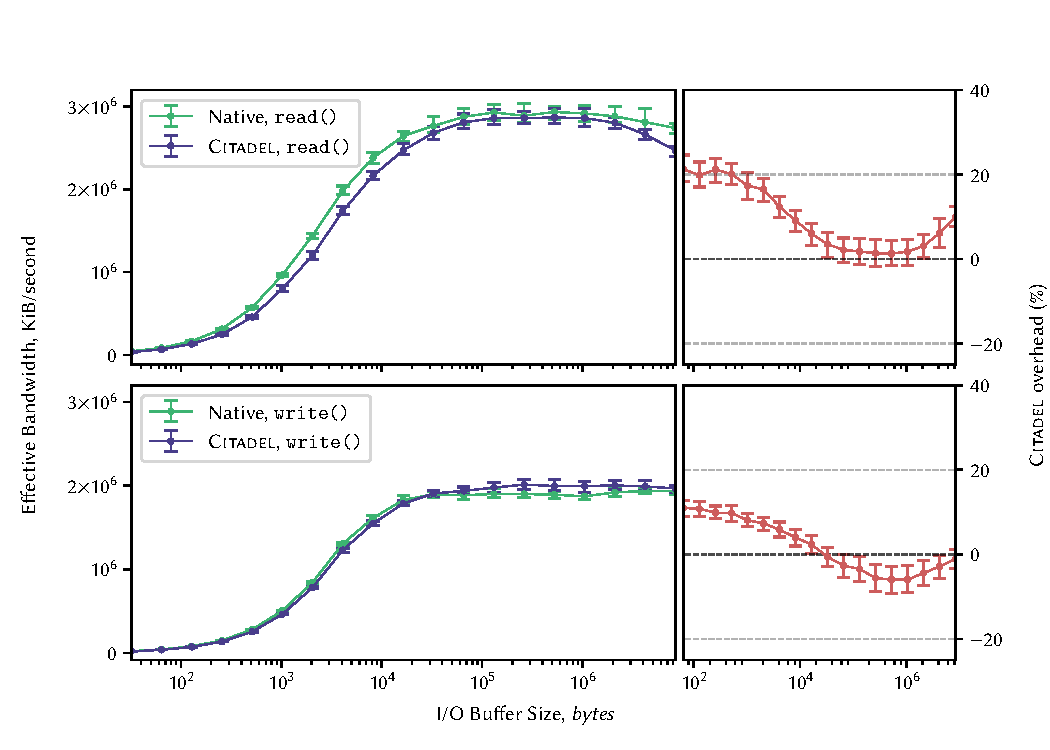
\includegraphics[width=\linewidth]{figures/graphs/io.pdf}
    \vspace{-5mm}
    \captionsetup{justification=centering}
    \caption[Effective \texttt{read()/write()} bandwidths for both the native Linux kernel and \textsc{Citadel}.]{Effective \texttt{read()/write()} bandwidths for both the native Linux kernel and \textsc{Citadel}. The percentage overhead is also presented. $n=200$.}
    \label{fig:io-graph}
\end{figure}


\begin{figure}[]
    \centering
    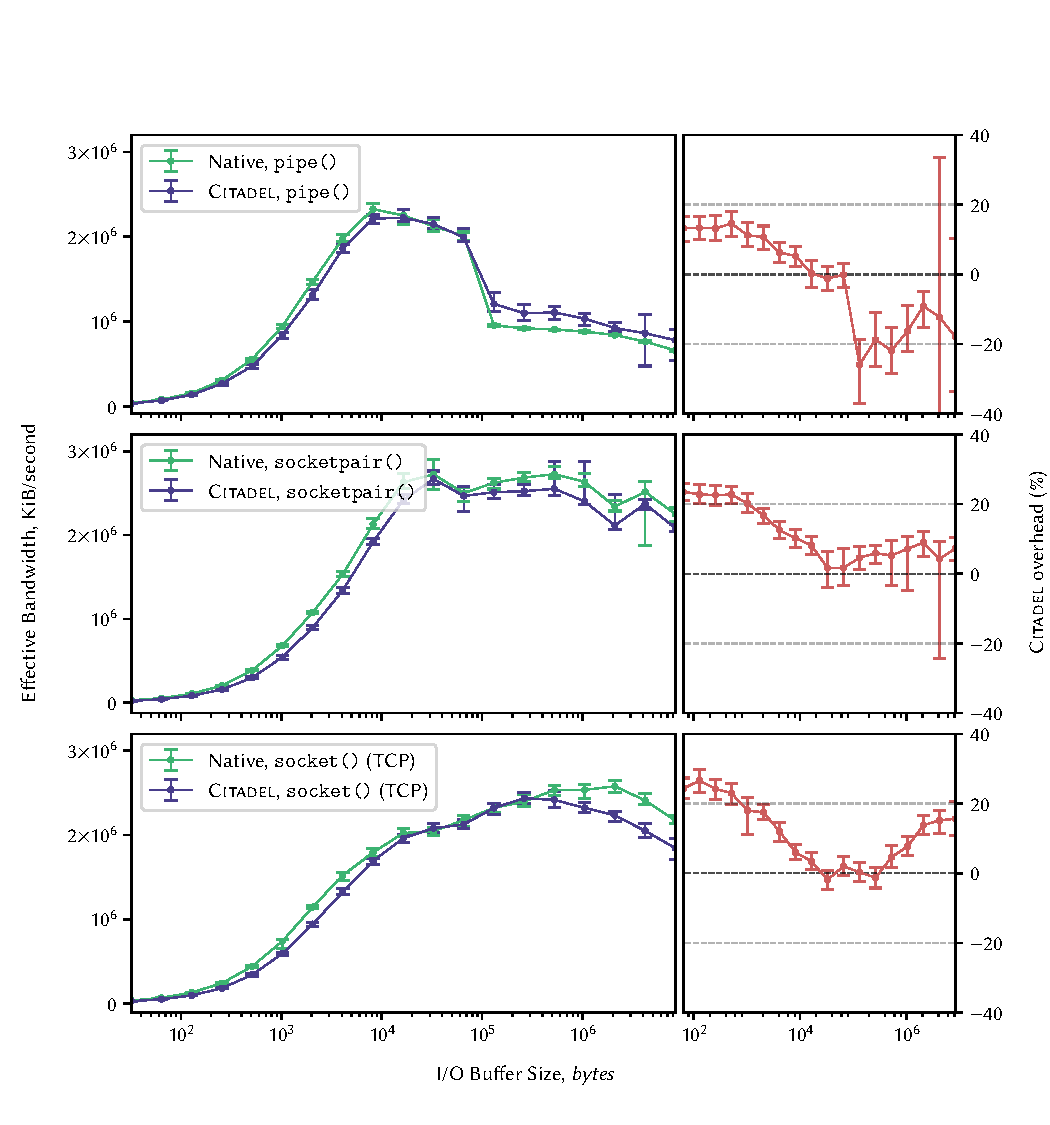
\includegraphics[width=\linewidth]{figures/graphs/ipc-2thread.pdf}
    \vspace{-5mm}
    \caption{Effective bandwidths for various types of IPC between \textit{2 threads}, $n=200$.}
    \label{fig:ipc-2thread-graph}
\end{figure}


\begin{figure}[]
    \centering
    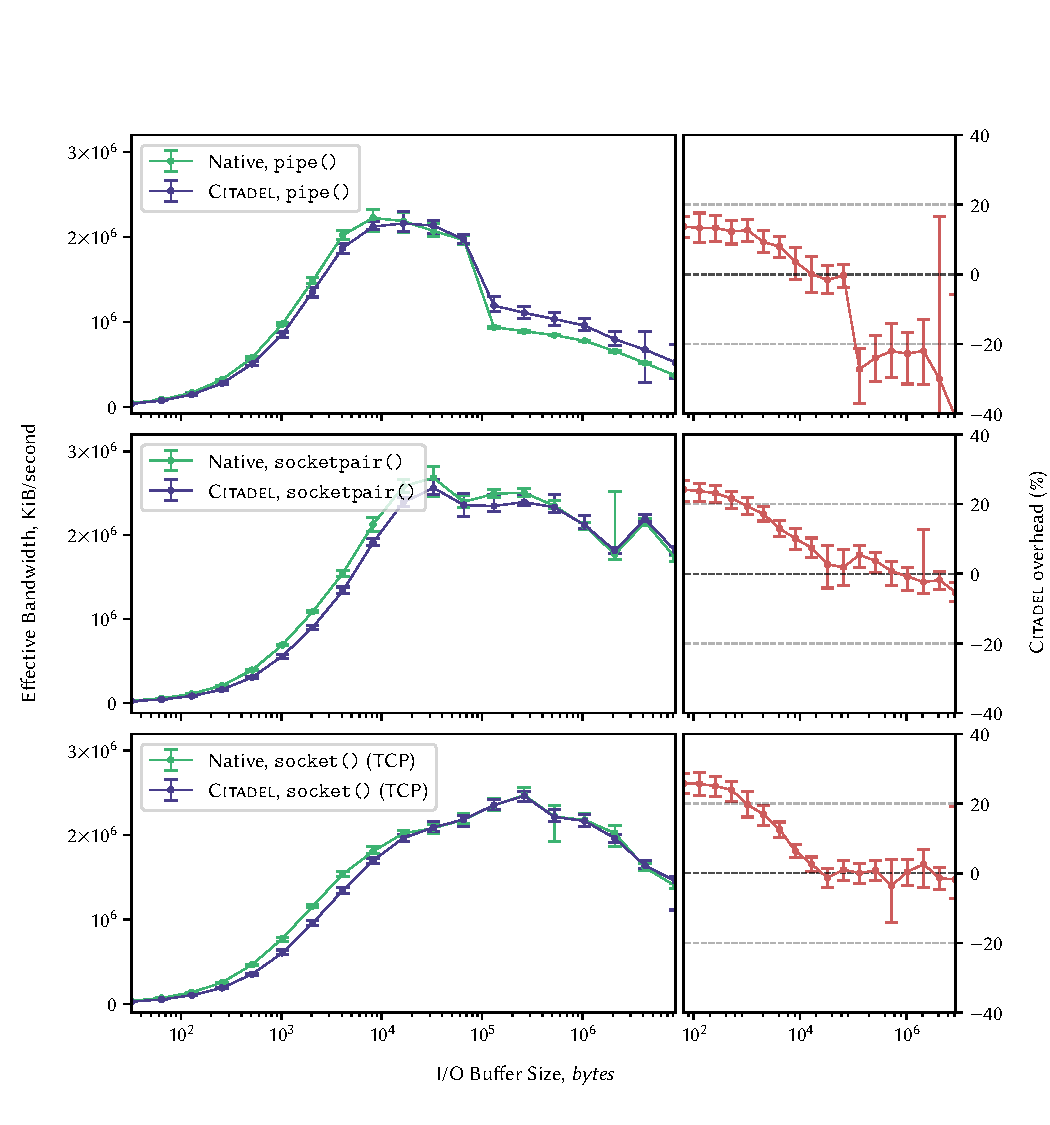
\includegraphics[width=\linewidth]{figures/graphs/ipc-2proc.pdf}
    \vspace{-5mm}
    \caption{Effective bandwidths for various types of IPC between \textit{2 processes}, $n=200$.}
    \label{fig:ipc-2proc-graph}
\end{figure}

\begin{figure}[]
    \centering
    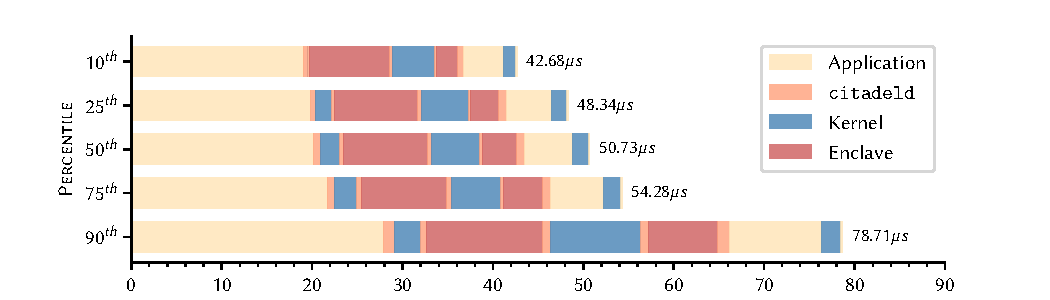
\includegraphics[width=\linewidth]{figures/graphs/open-anatomy.pdf}
    \vspace{-5mm}
    \caption{Control flow inhabitation for \texttt{libcitadel}'s \texttt{open()} function, $n=100$.}
    \label{fig:open-anatomy}
\end{figure}

\begin{table}
    \centering
    \newcommand\tableTop{\rule{0pt}{3ex}}
    \newcommand\tableMid{\rule{0pt}{3ex}}
    \newcommand\tableBottom{\rule[-2ex]{0pt}{0pt}}
    \newcolumntype{N}{>{\centering\arraybackslash}m{2.5in}}
    
    \renewcommand\theadfont{\normalsize}
    \renewcommand\arraystretch{1.3}
    \begin{tabular}{l@{\hskip 0.35in} r@{\hskip 0.3in} r@{\hskip 0.35in} r@{\hskip 0.35in} c} 
        
        \toprule
        & \thead{\multirow{2}{*}{\textsc{Native}}} & \multicolumn{3}{c}{\thead{\textsc{Citadel}}} \\
        \cline{3-5}
        &  & \thead{\textit{Untainted}} & \thead{\textit{Tainted}} & \thead{\textit{Overhead}} \\
        % \cline{1-4}
        \midrule 
        \multicolumn{5}{l}{\textsc{Webserver Benchmark}, \textit{100-byte packets}} \\
        \textit{Latency} & $35.73\mu s$ & $36.18\mu s$ & $44.35\mu s$ & $24\%$ \\
        $-\;$ \textit{std. dev.} & $13.85\mu s$ & $14.12\mu s$ & $13.26\mu s$ & \\
        $-\;$ \textit{max.} & $536\mu s$ & $554\mu s$ & $508\mu s$ & \\
        \textit{Requests/s} & $2.748 \cdot 10^4$ & $2.717 \cdot 10^4$ & $2.214 \cdot 10^4$ & $19\%$\\
        \textit{Bandwidth} & $177.28$ Mbps & $168.72$ Mbps & $143.04$ Mbps & $18\%$\\

        \midrule 
        \multicolumn{5}{l}{\textsc{10GB File Transfer}} \\
        \textit{Bandwidth} & $1.404$ Gbps & $1.410$ Gbps & $1.413$ Gbps & $\sim 0\%$ \\
        $-\;$ \textit{std. dev.} & $0.428$ Gbps & $0.440$ Gbps & $0.549$ Gbps &\\
        \textit{Duration} & $56.98 s$ & $56.74 s$ & $56.62 s$ & $\sim 0\%$ \\
        $-\;$ \textit{std. dev.} & $19.45 s$ & $18.97 s$ & $23.63 s$ & \\
        
        \bottomrule
    \end{tabular}

    \vspace{5mm}
    \captionsetup{justification=centering}
    \caption{\textsc{Nginx} performance comparinson between native Linux, and both untainted and tainted \textsc{Citadel}, $n=25$.}
\end{table}
